In the registration process the username and the password (sended with the encryption algorithm specified above) are written in the database.\\
Log in operation is required in order to use the functionalities of the system.
\\\\
When login happens the user inserts username and they are sended to the system; the system also obtains the ID device exploiting a GCM's function. In the DB several IDdevices can be associated to the same user, there is a field that marks the ID as mobile (related to phones and tablets) or browser (related to PCs). Browser IDs are deleted periodically. 
\\\\
The system behaves as specified in the flowchart according to the situation:
\begin{itemize}
\item first access: device is not present in the database;
\item login with different device: device is in the database, but it is associated to a different user;
\item login with the same device (not for the first time): a new univocal code is calculated and it will be update on the database.
\end{itemize}
The univocal code is a randomly generated string concatenated to the username (unique). The random string is calculated with the Current Unix Timestamp.
\\\\
The univocal code is sent to the device (a parameter that will be stored locally in the case of a mobile application, a cookie in the case of a browser) and will be used for every interaction with the system: in this way happens the identification of the user. For each request the system takes the univocal code received and the ID of the device and checks in the database if they are related.
\\
\begin{figure}
	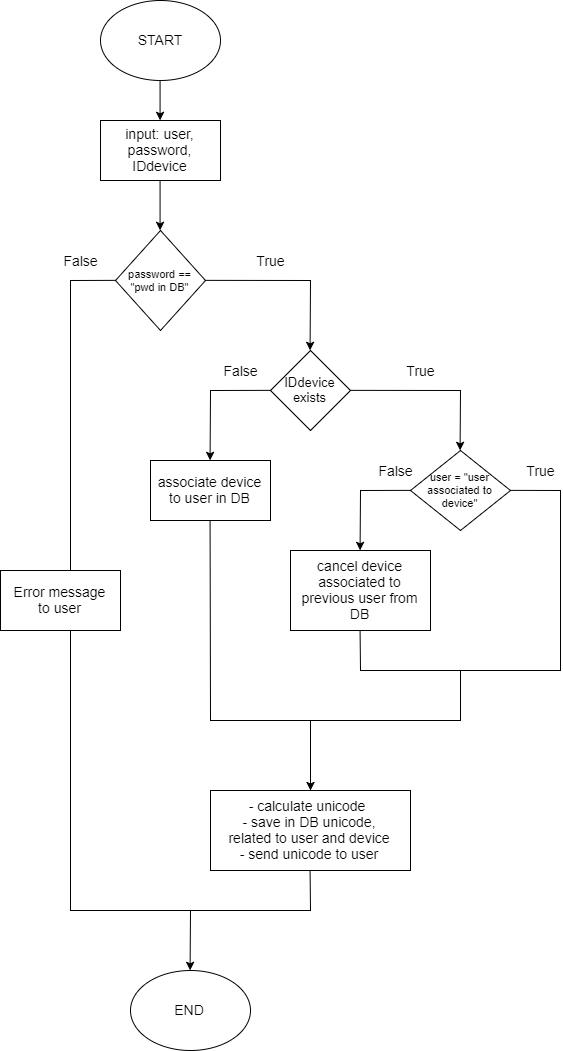
\includegraphics[scale=0.6]{algorithms/unicode_fc.png}
	\centering
	\caption{What happens during the login phase}
\end{figure}
